%1. Common problems and common technologies [+]
% - Text search +
% - Self Index +
% - Problems with self indexation +
% - Full text search with substrings +
%2. SA: overview, complexity, usage         [+]
%3. Radix: overview, complexity, usage      [+]
%4. Succinct data                           [+]
%5. CSA                                     [+]
%6. PSI                                     [+]
%7. Regenerating SA from PSI                [+]
%8. EF                                      [+]
%9. My CSA                                  []
%10.Complexity                              []

\textbf{Text retrieval}

Currently the Internet is updated with a large amount of data everyday.
That is why it is extremely important to organize search of necessary information in an \emph{effective} way.
In search within document indexing is applied.
\emph{Inverted index} is traditional for text indexing.
It is a data structure in which for each word in a document collection corresponding list
contains all the documents of a collection where this word is present.
While processing a multiple word request the intersection of lists is used,
that is corresponded to each word in a query.

\textbf{Problems of traditional approaches}

Some cases take place in practice where it is impossible to use
traditional full-text search by words \cite{bast2013efficient}.
A search model in which the task is to find orthographically close words (\emph{fuzzy search}),
that is used for spelling correction in numerous text editors,
does not allow one to solve the problem using full-text search.
The same applies to different systems where \emph{pattern matching} is used \cite{bai2018adaptive}.
Another example of texts where it is difficult to apply traditional search method
are several eastern languages.
In these languages words are not separated by spaces that makes \emph{inverted index} difficult to use.
Finally large texts combined from alphabet with a small amount of symbols can be attributed to <<inconvenient>> texts.
A typical example of these texts is DNA and protein structure code.
This text is not separated on words that is a key issue in using \emph{inverted index}.

To solve these problems it is necessary to perform substring search.
Existing methods (prefix tree, suffix array) take too much space therefore they are not effective.
For example, prefix tree that contains \emph{n} words with $C$ average number of symbols in a word
takes $O(n \cdot C)$ memory \cite{aho1975efficient}.
Let's take a greater look at suffix array as one of the most popular textual information indexation methods.

\textbf{Full-text search using suffix array}

Suffix array is a data structure used in full-text search that allows one to perform
substring search in a text consisting of \emph{n} symbols in $O(\log{}n)$ \cite{manber1993suffix}.
To store \emph{n} words in suffix array it is necessary to use $O(n \log{}n)$ of memory.
For instance, $2^{32}$ ASCII-text requires $2^{32} \cdot 8 = 32$ GB memory space.
For this text suffix array must contain 32 bit elements.
Therefore, suffix array size reaches $2^{32} \cdot 32 = 128$ GB memory space that is
4 times greater than the initial text size.

Suffix array is a sorted in a lexicographic order sequence of suffixes.
In order to better understand the structure of suffix array, consider this data structure
using as an example word <<mississippi>>:
\\(0) mississippi
\\(1) ississippi
\\(2) ssissippi
\\(3) sissippi
\\(4) issippi
\\(5) ssippi
\\(6) sippi
\\(7) ippi
\\(8) ppi
\\(9) pi
\\(10) i

Suffix array consisting of these suffixes would be presented as:

10 7 4 1 0 9 8 6 3 5 2

Usually the end of document is indicated by a special symbol that is not included in
the alphabet of a text stored in the array.
As a delimiter in this paper dollar symbol \$ has been chosen.
Modern approaches to suffix array construction allows one to  build data structure in $O(n)$.

\textbf{Radix tree}

% Picture By Claudio Rocchini - Own work, CC BY 2.5, https://commons.wikimedia.org/w/index.php?curid=2118795

\begin{wrapfigure}{r}{0.25\textwidth} %this figure will be at the right
 \centering
 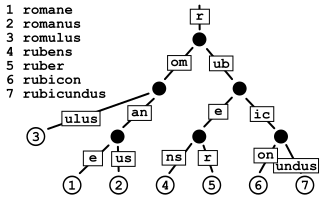
\includegraphics[width=0.45\textwidth]{PatriciaTrie}
 \caption{Radix tree example}
\end{wrapfigure}

Radix tree is a compressed prefix tree. In its turn, prefix tree is a data structure
that represents the intreface of associative array and allows one to store values in key-value pairs.
In this paper the string is chosen as a key, and in a contrary to regular trees,
the edges can contain either one element (symbol), or a sequence of elements (string).

Radix tree is commonly used in Linux kernel to bind a pointer with a long integer key \cite{Linux2018}.
This data structure is effective from the perspective of a search speed and data storage.
At the same time, Radix tree is used in IP-addressing because it is extremely useful for
hierarchical IP-addressing structure \cite{Radix2019} storage.

Let's take a detailed look at radix tree characteristics. Let us assume that it is required
to store keys the size of \emph{k} storing \emph{n} elements at the tree. Then insertion of an element,
search and removal take $O(k)$ operations \cite{leis2013adaptive}.

For many dictionary search requests radix tree can be faster and more effective than hash tables.
Despite the fact that often the complexity of search in a hash table is considered to be $O(1)$,
the necessity for the initial caching of input data is ignored in this assumption.
It takes $O(k)$ operations where \emph{k} is the length of input string.
Radix tree performs the search in $O(k)$, without initial data caching and has greater
cache localization characteristics.
It also preserves the order allowing one to perform an ordered scan,
get min / max values, scan over common prefix etc.

Because of all these advantages, radix tree is widely used in a Redis data base, program
products of HashiCorp, such as Terraform, Consul, Vault, Nomad etc \cite{Redis2018},
that is of additional interest for studying it on textual data and comparison with suffix array.

\textbf{Succinct data representation}

One of the most important problems of this research is
a program implementation of succinct index storage for suffix array.
That is why it is important to understand what data can be considered succinct.

There are several degrees of information compression.
Let us assume that the storage of a piece of data takes \emph{Z} bit.
Succinct data structures take \(Z + o(Z)\) bit, implicit -- \(Z + o(1)\) bit and
compact -- \(O(Z)\) bit \cite{huo2014practical}. In this paper it is proposed to
compress suffix array in succinct data representation.
Thus, the size of array is only a little bit greater than the size of initial text.

\textbf{$\Psi$-array}

An important part in a theory of succinct index representation is taken by an intermediate $\psi$-array.
A characteristic feature of all the compression algorithms of a compressed suffix array (CSA) is 
that not the index itself is compressed but it's representation as a $\psi$-array.
Auxiliary array can be obtained from suffix array by the following index manipulations.
Let us consider a $\psi$-array construction by the example of a familiar string \textbf{mississippi\$}:
\\ \textbf{Text}:\,\,\,\,\,\,\,\,\,\,\,\,\,\,\,\,\,\,\,\,\,\,\,\, m \,i \,\,\,\,s \,\,\,s \,\,\,\,i \,\,\,\,s \,\,\,s \,\,i \,\,p \,\,p \,\,i \,\,\,\,\$
\\ \textbf{Offset}:\,\,\,\,\,\,\,\,\,\,\,\,\,\,\,\,\,\,\,\, 0 \,\,1 \,\,\,\,2 \,\,3 \,\,\,4 \,\,\,5 \,\,6 \,7 \,\,8 \,\,9 \,10 11
\\ \textbf{Suffix Array}:   11 10 \,7 \,\,4 \,\,\,1 \,\,\,0 \,\,9 \,8 \,\,6 \,\,3 \,\,5 \,\,2
\\ \textbf{$\Psi$ -array}: \,\,\,\,\,\,\,\,\,\,\,\,\$ \,\,\,0 \,\,\,\,7 10 \,\,11 4 \,\,1 \,6 \,\,2 \,\,3 \,\,8 \,\,9

Let us call the largest suffix of a substring except for the initial string as a successor.
Therefore, for substring issippi\$ successor is ssippi\$.
$\Psi$-array points out to a successor for every chosen suffix.
As an example consider $SA[7] = 8$. It's successor is a position in a suffix array that contains $8 + 1 = 9$.
Thus, $\psi[7] = 6$. The main relation between a $\psi$-array and suffix array:
\begin{equation}\label{sa:1}
SA[i] = SA[\psi[i]] - 1
\end{equation}
It is necessary to emphasize that $\Psi[0] = \$$, because there is no successor for the first element in a suffix array.
However, $SA[5]$ is reffered to 0 index, that is the whole string overall.
In other words, the element of suffix array is reffered to the beginning of the text,
that is no other suffix can have it as a child.
There is no element equal to 5 in a $\psi$-array, respectively.

\textbf{Suffix array reconstruction from a $\psi$-array}

There is an opportunity to reconstruct the initial suffix array by generated $\psi$-array
with operations that are reversive to those that were present in the last paragraph.
Let us have a better look at the specific features of this algorithm.

First of all, it is necessary to find the index of the element of suffix array that has not been present in the $\psi$-array.
In our example it is equal to 5. From the discussions above, it can be seen that $SA[5] = 0$.
Thus, one element of an initial suffix array was reconstructed. From the formula \ref{sa:1} for $i = 5$ follows:

\[SA[5] = SA[\psi[5]] - 1\]
\[0 = SA[4] - 1\]
\[SA[4] = 1\]

Another element of a suffix array is reconstructed!
This way the whole remaining sequence can be reconstructed.
Time taking to find the first element is equal to \(O(n)\) operations.
There are several improvements of the search speed of a certain elements in a suffix array
that require additional data structures storing suffix array values at every \(\log n\) step \cite{andersensimple}.
This approach goes beyond this paper, because the main problem of it is to find the best index compression.







\textbf{Сжатие $\psi$-массива}

Рассмотрим подробнее $\psi$-массив:
\\ \textbf{Text}:\,\,\,\,\,\,\,\,\,\,\,\,\,\,\,\,\,\,\,\,\,\,\,\, m \,i \,\,\,\,s \,\,\,s \,\,\,\,i \,\,\,\,s \,\,\,s \,\,i \,\,p \,\,p \,\,i \,\,\,\,\$
\\ \textbf{Offset}:\,\,\,\,\,\,\,\,\,\,\,\,\,\,\,\,\,\,\,\, 0 \,\,1 \,\,\,\,2 \,\,3 \,\,\,4 \,\,\,5 \,\,6 \,7 \,\,8 \,\,9 \,10 11
\\ \textbf{Suffix Array}:   11 10 \,7 \,\,4 \,\,\,1 \,\,\,0 \,\,9 \,8 \,\,6 \,\,3 \,\,5 \,\,2
\\ \textbf{$\Psi$ -array}: \,\,\,\,\,\,\,\,\,\,\,\,\$ \,\,\,0 \,\,\,\,7 10 \,\,11 4 \,\,1 \,6 \,\,2 \,\,3 \,\,8 \,\,9

Отсортированный набор суффиксов имеет вид:
\\ (0) \,\,\,\$
\\ (1) \,\,\,i\$
\\ (2) \,\,\,ippi\$
\\ (3) \,\,\,issippi\$
\\ (4) \,\,\,ississippi\$
\\ (5) \,\,\,mississippi\$
\\ (6) \,\,\,pi\$
\\ (7) \,\,\,ppi\$
\\ (8) \,\,\,sippi\$
\\ (9) \,\,\,sissippi\$
\\ (10) ssippi\$
\\ (11) ssissippi\$

Стоит обратить внимание на его структуру: он состоит из набора возрастающих последовательностей индексов.
Рассмотрим возрастающую последовательность 2, 3, 8, 9.

$SA[2] = 7$, $T[7] = i$.
$SA[3] = 4$, $T[4] = i$. Примечательно, что $SA[6] = 9$, $T[9] = p$.
То есть чередование индексов с возрастания на убывание соответствует смене символа с i на p.

\begin{theorem}
 \label{lemma:1}
 Два последовательных элемента $\psi$-массива являются возрастающими, если соответствующие суффиксы,
 на которые они ссылаются, начинаются с одного и того же символа.
\end{theorem}

\begin{proof}
 По построению, suffix array представляет собой набор индексов в исходном тексте,
 отсортированный в лексикографическом порядке. Это означает, что $T[SA[i]] < T[SA[i + 1]]$
 $\forall i \in [0, n).$ Эти два суффикса имеют общий первый символ. Поэтому они отличаются в следующих
 элементах, например, во втором: $T[SA[i] + 1] < T[SA[i + 1] + 1].$

 $\Psi$-массив ссылается на потомка для данного суффикса: $T[SA[\psi[i]]] < T[SA[i] + 1].$
 Т.к. $T[SA[i]]$ и $T[SA[i + 1]]$ имеют одинаковый первый символ, их потомки упорядочены.
 Если $T[SA[\psi[i]]] < T[SA[\psi[i + 1]]]$, тогда из-за упорядоченности индекс в suffix array
 для первого должен находиться перед индексом для второго. Следовательно индексы (значения $\psi$-массива)
 должны быть упорядочены, если суффиксы имеют общий первый символ.
\end{proof}

Возрастающие последовательности неотрицательных целых чисел сжимаемы \cite{andersensimple}.
Самый простой путь для хранения таких последовательностей -- битмап.
Однако этот способ не позволяет иметь произвольный доступ к элементам.
Рассмотрим более совершенный алгоритм сжатого представления данных.

\textbf{Кодировка Elias--Fano}

Сжатие при помощи метода Elias--Fano \cite{pibiri2014dynamic}
позволяет представлять монотонно возрастающие последовательности
целых неотрицательных чисел в виде битовых векторов. Этот способ делает возможным
хранение неубывающей последовательности $n$ целых чисел размером $[0, m)$,
занимая $2n + n[\log m/n]$ бит, предоставляя доступ к $i$-му элементу за $O(1)$.
Сравнив размеры структуры данных с минимально возможным занимаемым местом в памяти
с точки зрения теории информации, Elias--Fano кодировка является сжатым (succinct) индексом.

\begin{figure}[t]
 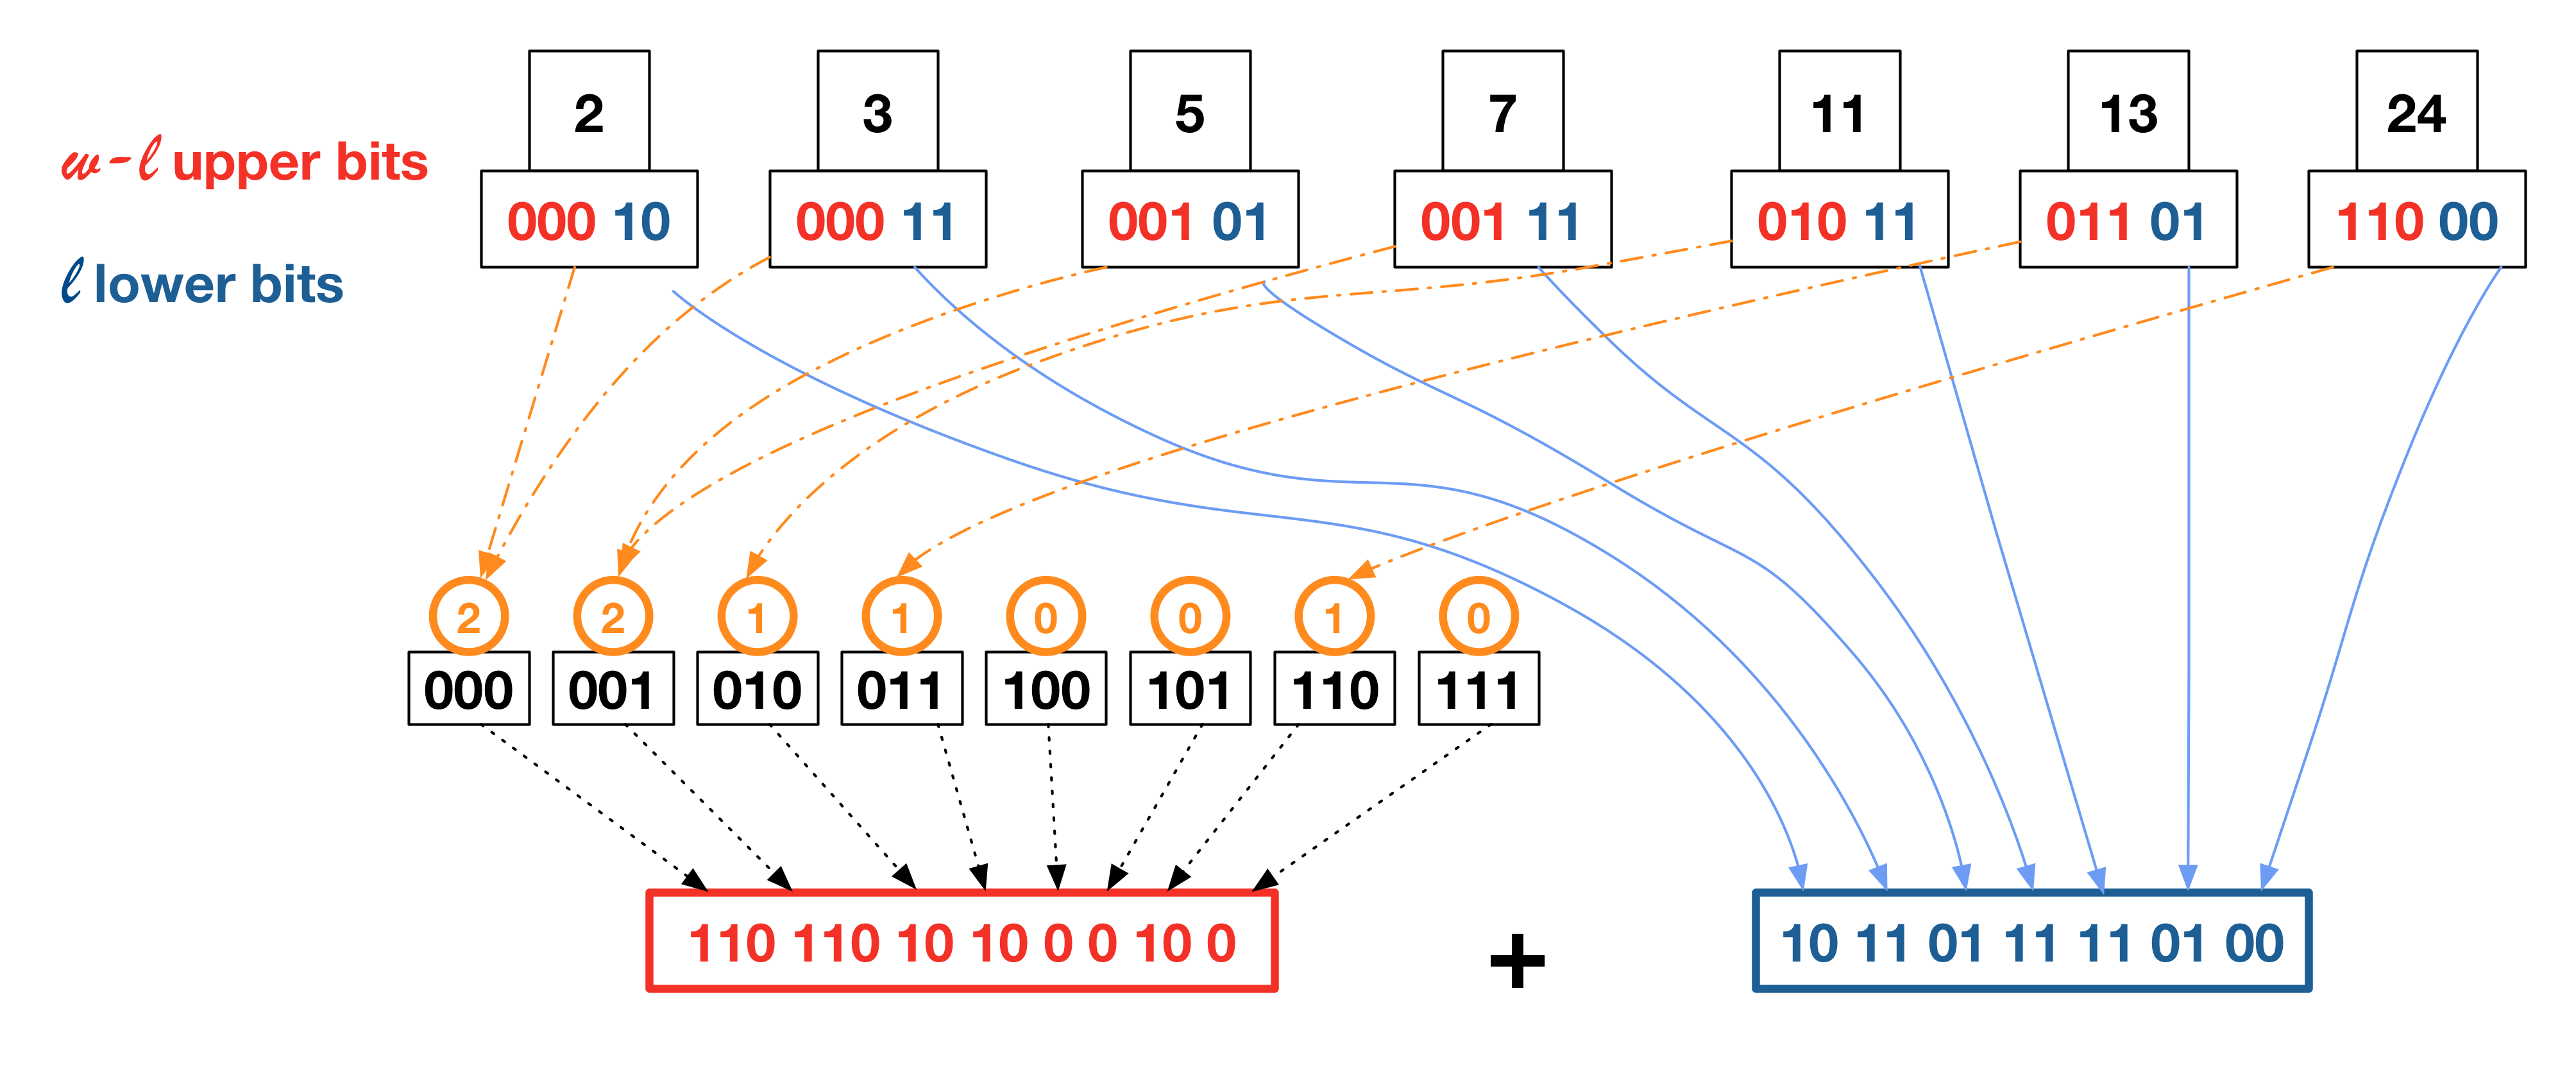
\includegraphics[width=12cm]{Elias-Fano}
 \caption{Пример построения кода Elias-Fano}
 \centering
 \label{fig:EF}
\end{figure}

В начале каждое число из последовательности кодируется $\log m$ битами данных.
Двоичное представление элементов разбито на две части: верхнюю часть, содержащую в себе
первые $\log n$ бит, и нижнюю, с оставшимися $\log m - \log n = \log m / n$ бит.
Объединение нижних битов занимает $n \log m$ бит. Верхние биты представляют собой
набор из $n + m / 2^{\log m/n}$ бит \cite{antonio2018integers}.
Начиная с пустого битового вектора, мы добавляем в эту часть 0
в качестве стоп-бита для каждого возможного значения, представляемого битами старшей части.
Мы добавляем 1 для каждого фактически присутствующего значения, выставляя его перед соответствующим стоп-битом.

В качестве примера рассмотрим отсортированную последовательность {2,3,5,7,11,13,24}.
На рисунке \ref{fig:EF} показана схема кодирования. Наибольшим числом в наборе (universe) является 24.
Поэтому для представления каждого элемента необходимо выделить 5 бит на элемент.
Затем нужно разбить бинарное представление на две части: верхнюю и нижнюю.
Исходя из ранее оговоренных условий, выберем 3 бита под верхнюю часть и 2 бита под нижнюю.
Всего в последовательности присутствует 7 элементов. Рассмотрим число 2. Для него имеем
$2 = 0b00010$ и соответственно 000 в качестве верхней части и 10 в качестве нижней.
Повторяя этот процесс, получим набор нижних частей для каждого элемента.
Затем объединим полученные части вместе. Для верхних частей имеется $2^3$ вариантов
наборов значений. С каждым таким набором ассоциируется счетчик, который увеличивается на единицу,
если число из последовательности имеет соответствующую верхнюю часть.
Так для 2 инкрементируем набор 000. Число $3 = 0b00011$ с верхней частью 000 идет в тот же набор.
Для числа $5 = 0b00101$ с верхней частью 001 инкрементируем набор 001 и т.д.
Наконец, кодируем счетчики унарно, добавляя столько единиц в представление счетчика,
сколько имеет значение каждого счетчика, за которым следует 0 бит.
Окончательное кодирование Elias-Fano получается объединением полученных верхней и нижней частей.

\textbf{Восстановление данных из кода Elias--Fano}

Для восстановления исходной монотонной неубывающей последовательности чисел, необходимо разработать операцию
доступа к $i$-му элементу последовательности, $i \in [0, n)$. Для доступа к нижней части
достаточно просто получить соответствующие биты, т.к. длина вектора для хранения элемента известна.
Для получения старшей части, необходимо осуществить операцию \emph{select}.
Операция \emph{select($i$)} позволяет получить позицию $i$-го бита, выставленного в 1 в битовом векторе.
Эта операция может быть выполнена за $O(1)$, что позволяет получать произвольный доступ к элементу
последовательности без полного раскодирования всей последовательности целиком \cite{farina2009rank}.